\documentclass[a4paper, 12pt]{article}
\usepackage{a4wide}
\usepackage{amsmath}
\usepackage{graphicx}
\usepackage{hyperref}
\usepackage{cite}
\usepackage{bbm}

\title{Strategy for Share Buyback with Reinforcement Learning and Pre-training to different type of share repurchasing}
\author{Mark-Killian Zinenberg \\ DVRC Esilv}
\date{January 2025}
\begin{document}

\maketitle

\begin{abstract}
This paper presents a machine learning approach for the management of share buyback contracts, focusing on addressing the challenges posed by high-dimensional state spaces. Unlike conventional methods, such as grid-based or tree-based approaches, which often face limitations due to the curse of dimensionality, our framework employs reinforcement learning to optimize decision-making for buyback strategies, with a primary focus on accelerated share repurchase (ASR) contracts. While the proposed methodology successfully replicates strategies found in existing literature, further refinements are needed to address remaining challenges and improve robustness.
\end{abstract}

\section{Introduction}
Companies buy back stock for many different reasons. Executives cite undervaluation of the company’s stock, signaling, financial flexibility, availability of excess cash, and risk
management as some important drivers of their stock buyback decisions [4],[5]. ASRs have become the second most popular method of share repurchases in the US [9], as they allow companies to repurchase shares quickly and efficiently especially motivated by undervaluation of the company’s stock. [10] 

The objective of this project is to model and optimize a share buyback strategy using reinforcement learning. We studied various approaches, including the Stochastic Policy Gradient method [1], and explored several techniques and neural network architectures to enhance the agent's decision-making process.

Our work involved a thorough review of relevant academic literature [1],[2],[3], as well as the implementation and experimentation of multiple algorithms. While the preliminary results are encouraging, some limitations remain, and we outline here the challenges encountered along with potential areas for improvement.

Among the aspects not covered in the literature are:

Dimensionality reduction to three variables for ASR contracts.
More complex VWAP-minus programs, such as profit-sharing participation programs.
Due to the high-dimensional nature of the problem [6], it is natural to address the pricing and management of ASRs and other, more complex VWAP-minus programs using neural networks instead of grids or trees [5].

This study, therefore, focuses on different possible payoffs:

ASR with a fixed number of shares,
ASR with fixed-rate contracts,
Notional and profit-sharing contracts.

For now, we are limiting our scope to accelerated share repurchase (ASR) contracts. [11,12,13]

The methodology section describes the stock buyback environment (subsection 2.1), the agent's architecture (subsection 2.2), the payoff calculation (subsection 2.3), and the training process (subsection 2.4). The results section presents the findings of the research, including figures and analyses. The discussion section outlines the challenges encountered and potential areas for improvement. The conclusion section summarizes the key takeaways and outlines future research directions.

\section{Methodology}

\subsection{The environment}
The goal is to buy a specific number of stocks over a given period. The stock prices fluctuate daily, and the agent is tasked with deciding the optimal number of stocks to purchase each day. The agent receives the following states:
\begin{itemize}
    \item Historical prices $S_n$
    \item Mean of prices over time $A_n$
    \item The current day $n$
    \item Total stock purchased and total spent
\end{itemize}

The agent can trigger a bell signal to stop the process once the goal is achieved.

The Initial Stock Price is $S_0 = 45$ and the Stock Price Dynamics is given by: \\ $S_{n+1} = S_n + \sigma X_{n+1}$, where $X_n \sim \mathcal{N}(0, 1)$. \\ We also need the Average Price given by $A_n = \frac{1}{n} \sum_{k=1}^{n} S_k$ then the Price paid for buying $v_n$ stocks is $v_n \cdot S_{n+1}$.\\  The nuance is that after Day 22, a bell can be rung when the goal is met which we call here the stopping time. \\ In first attempt, we chose to fix these parameters: We chose to set a fixed volatility \( \sigma = 0.6 \) and a fixed goal of 20 stocks to buy over 63 days.
\\ 
\textbf{Initial objective:} Maximize the total payoff:
\[
\text{payoff} = \text{goal} \times A_n - \text{total spent}
\]


\subsection{Agent Model Definition}

The agent is modeled using a neural network defined by the \texttt{StockNetwork} class. The neural network has the following characteristics:

\begin{itemize}
    \item \textbf{Inputs}: The current state \( (n, S_n, A_n, q_n, X_n) \), where:
    \begin{itemize}
        \item \( n \) indicates the current day of the simulation.
        \item \( S_n \) is the current stock price.
        \item \( A_n \) is the average stock price up to day \( n \).
        \item \( q_n \) is the total number of stocks held.
        \item \( X_n \) is the amount spent on purchasing stocks.
    \end{itemize}
    \item \textbf{Outputs}: The agent outputs a tuple \( (\text{TotalStockTarget}, \text{Stopping decision}) \), where:
    \begin{itemize}
        \item \( \text{TotalStockTarget} \) is the target number of stocks to buy, sampled from a normal distribution.
        \item \( \text{Stopping decision} \) is a binary decision parameter, indicating whether it is appropriate to stop buying stocks after reaching \( Q \).
    \end{itemize}
\end{itemize}

The agent follows a stochastic policy, where the number of stocks to purchase is sampled from a normal distribution with a mean calculated by the model and a standard deviation proportional to the buyback \( Q \). The policy is given by:
\[
\text{TotalStockTarget} \sim \mathcal{N}(\mu_n, \sigma_n)
\]
where \( \mu_n \) is the average number of stocks to buy returned by the agent, and \( \sigma_n \) is the standard deviation defined by \( \frac{Q}{\text{days}} \cdot 0.05 \) to allow exploration.

In addition, the agent employs a Bernoulli distribution for its "Stopping decision" parameter. The decision-making process for this parameter is as follows:

\begin{itemize}
    \item Sampling from a Bernoulli distribution is used to determine whether the "Stopping decision" action should be activated.
    \item The cumulative distribution function \( F(x) \) of the Bernoulli distribution is defined as:
    $F(x) = 0 \cdot \mathbbm{1}_{\{x < 0\}} + (1 - p) \cdot \mathbbm{1}_{\{0 \leq x < 1\}} + 1 \cdot \mathbbm{1}_{\{x \geq 1\}}$
    where \( p \) is the probability of activation.
    \item The sampling mechanism involves inverting the cumulative distribution function:
    \[
    1 - u = U \sim \text{Unif}(0,1)
    \]
    where \( U \) is a uniform random variable. The "Stopping decision" parameter is then computed as:
    \[
    \text{Stopping decision} = \begin{cases}
    1 & \text{if } u < \text{Stopping decision\_param}, \\
    0 & \text{otherwise}.
    \end{cases}
    \]
\end{itemize}

By combining the outputs from the neural network, the agent generates two key parameters:
\begin{itemize}
    \item \( \text{TotalStockTarget} \), sampled from \( \mathcal{N}(\mu_n, \sigma_n) \), where \( \mu_n \) is the mean and \( \sigma_n = \frac{Q}{\text{days}} \cdot 0.05 \).
    \item \( \text{Stopping decision} \), determined by comparing a uniformly drawn random variable \( u \) against the network's output.
\end{itemize}

This implementation allows the agent to adaptively respond to market conditions, optimizing the buyback process by balancing exploration and exploitation.


\subsection{Payoff Calculation}

Initially, the payoff is calculated only at the end of the episode: when the agent decides to ring the Stopping decision and the total number of stocks reaches Q or after a set number of days. The payoff function is defined as:
\[
\text{payoff} = Q \cdot A_n - X_n
\]
where \( A_n \) is the average stock price at the end of the episode, \( X_n \) represents the amount spent on purchasing the stocks, and Q represents the total number of stocks to buy.

On the other hand, we can compute the expected payoff using the law of total expectation and recursive chains of expectations. This approach captures the influence of the agent's decisions at each step of the episode, taking into account both immediate and future outcomes.

At each step \( n \) in the episode, the agent makes a decision on whether to continue purchasing stocks or stop, based on the Stopping decision signal \( \text{Stopping decision}_n \), which follows a Bernoulli distribution. The expected payoff at each step is conditioned on whether the Stopping decision rings (\( \text{Stopping decision}_n = 1 \)) or not (\( \text{Stopping decision}_n = 0 \)).

The expected payoff at step \( n \), conditioned on \( \text{Stopping decision}_n \), is given by:
\[
\mathbbm{E}[\text{payoff}_n] = \text{payoff}_n \cdot \text{Stopping decision}_n + (1 - \text{Stopping decision}_n) \cdot \mathbbm{E}[\text{payoff}_{n+1}]
\]
Where:
\begin{itemize}
    \item \( \text{payoff}_n \) is the immediate payoff at step \( n \),
    \item \( \text{Stopping decision}_n \) indicates whether the agent stops or continues at step \( n \),
    \item \( \mathbbm{E}[\text{payoff}_{n+1}] \) is the expected payoff at the next step \( n+1 \), which depends on future decisions.
\end{itemize}

By applying the law of conditional expectation recursively across all steps of the episode, the total expected payoff is calculated step by step, where each payoff depends on both the current and future decisions. The recursion starts from the final step \( N \) and works backward to the first step:

\[
\mathbbm{E}[\text{payoff}_N] = \text{payoff}_N \cdot \text{Stopping decision}_N
\]
\[
\mathbbm{E}[\text{payoff}_{N-1}] = \text{payoff}_{N-1} \cdot \text{Stopping decision}_{N-1} + (1 - \text{Stopping decision}_{N-1}) \cdot \mathbbm{E}[\text{payoff}_N]
\]
\[
\mathbbm{E}[\text{payoff}_{N-2}] = \text{payoff}_{N-2} \cdot \text{Stopping decision}_{N-2} + (1 - \text{Stopping decision}_{N-2}) \cdot \mathbbm{E}[\text{payoff}_{N-1}]
\]
This recursive process continues until we reach the first step \( n = 1 \), where the total expected payoff is:

\[
\mathbbm{E}[\text{payoff}_1] = \text{payoff}_1 \cdot \text{Stopping decision}_1 + (1 - \text{Stopping decision}_1) \cdot \mathbbm{E}[\text{payoff}_2]
\]

The total expected payoff across the entire episode can be written as a recursive chain of conditional expectations, starting from the first step \( n = 1 \) and summing up the contributions from all steps:

\[
\mathbbm{E}[\text{payoff}_1] = \sum_{n=1}^{N} \left( \prod_{i=1}^{n-1} (1 - \text{Stopping decision}_i) \right) \cdot \left( \text{payoff}_n \cdot \text{Stopping decision}_n \right)
\]

In this formula:
\begin{itemize}
    \item \( \prod_{i=1}^{n-1} (1 - \text{Stopping decision}_i) \) is the cumulative probability that the agent reaches step \( n \) without the Stopping decision ringing at any previous step,
    \item \( \text{payoff}_n \cdot \text{Stopping decision}_n \) is the immediate payoff at step \( n \), weighted by whether the agent stops or continues at that step.
\end{itemize}

This approach allows us to calculate the total expected payoff by recursively chaining the expected payoffs across all steps in the episode, capturing both the immediate payoffs and the influence of future decisions.

The recursive chain of expectations ensures that each step of the episode is accounted for in the total expected payoff, with each step conditioned on whether the agent stops or continues at each decision point. This method provides a more detailed and accurate representation of the agent's performance over the course of the episode, by integrating both immediate and future payoffs.


\subsection{Policy Gradient Learning Algorithm}

The agent's parameter update is based on the calculation of the \textit{log-density} of the actions taken. First, we calculate the probability density functions (pdf) for both actions. The pdf for the total stock target, assuming it follows a normal distribution, is given by:
\[
\text{pdf\_total\_stock\_target} = \frac{1}{\sqrt{2\pi\sigma_n^2}} \exp\left(-\frac{(TotalStockTarget - \mu_n)^2}{2\sigma_n^2}\right)
\]
The pdf for the Stopping decision action is calculated based on the Stopping decision parameter:
\[
\text{pdf\_Stopping decision} = \begin{cases} 
Stopping decision\_param & \text{if } Stopping decision = 1 \\ 
1 - Stopping decision\_param & \text{if } Stopping decision = 0 
\end{cases}
\]

Once we have the pdfs, we can compute the log-densities of the actions. The log-density for the total stock target is:
\[
\log p(TotalStockTarget | \mu_n, \sigma_n) = -\frac{1}{2} \left( \frac{(TotalStockTarget - \mu_n)^2}{\sigma_n^2} + \log(2\pi\sigma_n^2) \right)
\]
The log-density of the Stopping decision action is:
\[
\log p(Stopping decision | Stopping decision\_param) = \log(\text{pdf\_Stopping decision})
\]

The overall log-likelihood for the agent's actions can then be expressed as:
\[
\log(\text{density}) = \log(\text{pdf\_Stopping decision}) + \log(\text{pdf\_total\_stock\_target})
\]

This log-density reflects the independence of actions, allowing us to express the total log-likelihood as the sum of the log-densities of the marginal actions. This is crucial for the parameter update during training, where the log-likelihood facilitates the gradient calculation.

During training over multiple batches, the gradients are accumulated, and the loss is computed as follows:
\[
\text{loss} = -\left( \sum \log(\text{density}) \cdot \text{episode\_payoff} \right) / N
\]
where \( N \) is the number of batches. The agent's parameters \( \theta \) are updated by maximizing the expected payoff using the policy gradient method:
\[
\theta \leftarrow \theta + \alpha \nabla_\theta \log p(TotalStockTarget | \mu_n, \sigma_n) \cdot \text{payoff}
\]
where \( \alpha \) is the learning rate.



\section{Results}
Here is a graph of the agent's decisions over time, showing the stock buyback process and the agent's actions at each step for 2 batches. The agent's decisions are based on the neural network's outputs, which determine the number of stocks to purchase and whether to ring the Stopping decision.
\begin{figure}
    \centering
    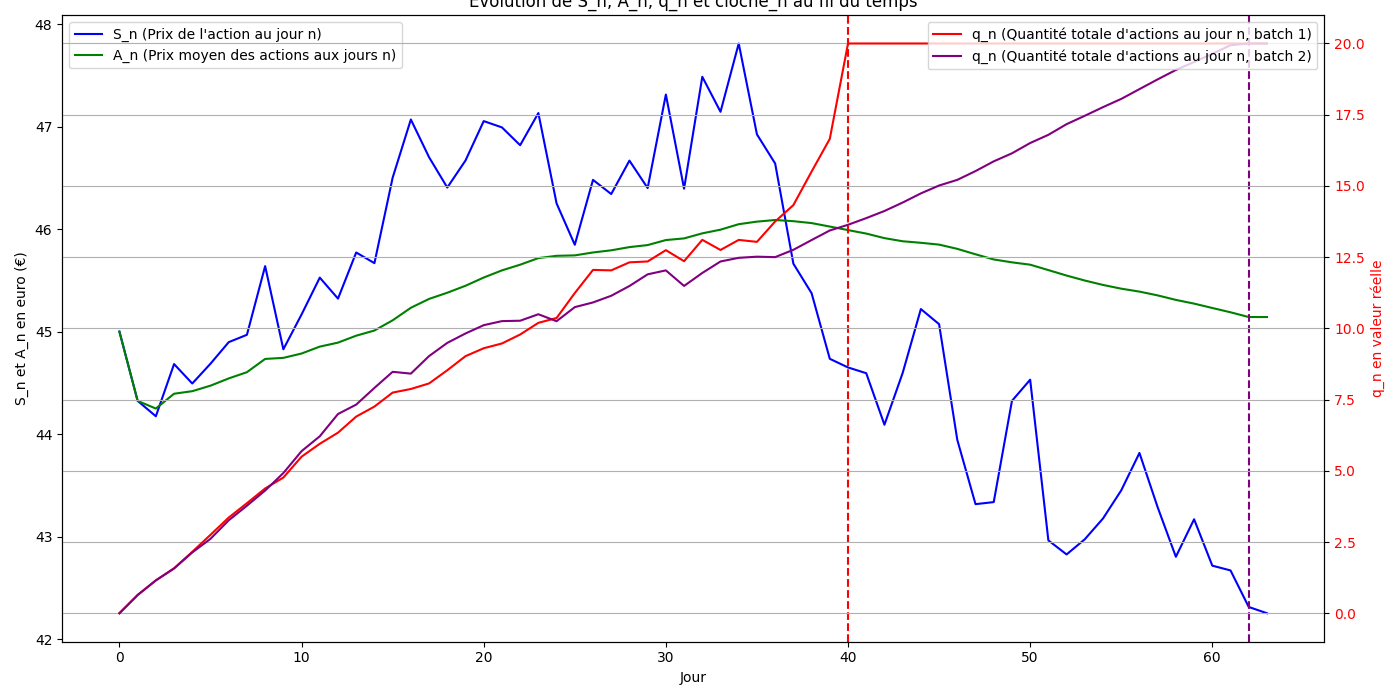
\includegraphics[width=1\textwidth]{Net evaluation.png}
    \caption{Visualisation of the stock buyback process and agent's decisions over time.}
\end{figure}
\begin{figure}
    \centering
    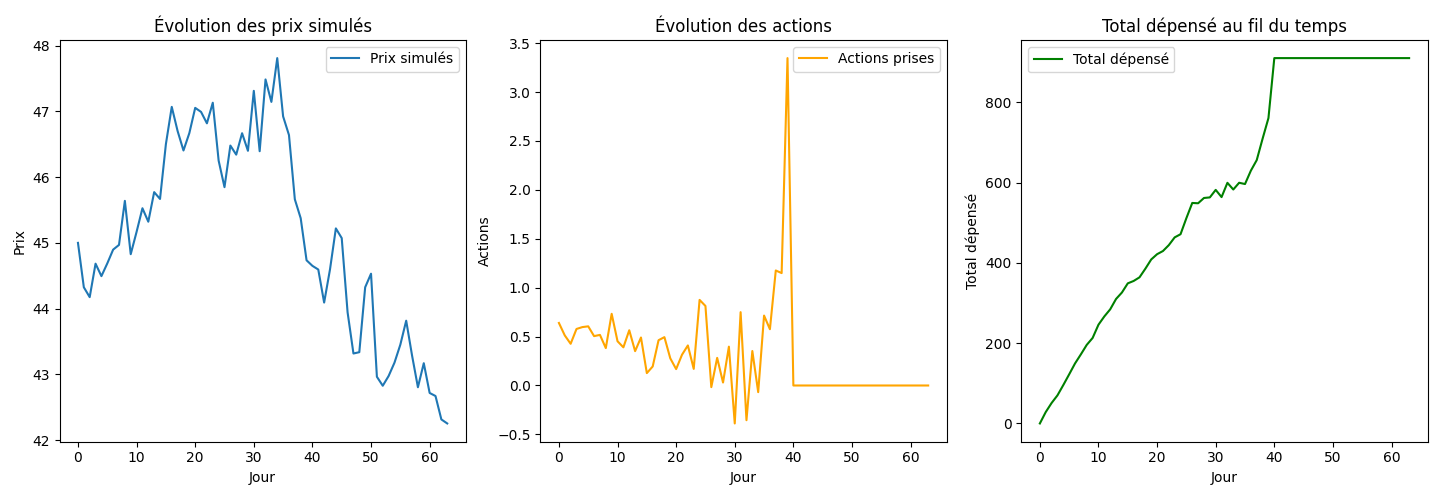
\includegraphics[width=1\textwidth]{Net evaluation autre graphes.png}
    \caption{Another visualisation of another iteration}
\end{figure}

\subsection{Impact of Volatility}
In this experiment, we varied the volatility parameter $\sigma$ to analyze its impact on the agent's decision-making process and overall performance. The graph above illustrates how changes in volatility influence the stock buyback strategy. Higher volatility increases uncertainty in stock prices, prompting the agent to adopt either a more conservative or aggressive buying approach. The results demonstrate the agent's ability to adapt its strategy based on volatility levels, showcasing the robustness of the reinforcement learning framework in navigating diverse market conditions.

We observe that as volatility increases, the agent tends to trigger the stopping decision earlier, reflecting the heightened difficulty of accurately predicting future stock prices. This behavior underscores the agent's adaptability in the face of greater market uncertainty, further highlighting the flexibility and effectiveness of the reinforcement learning approach.
\begin{figure}
    \centering
    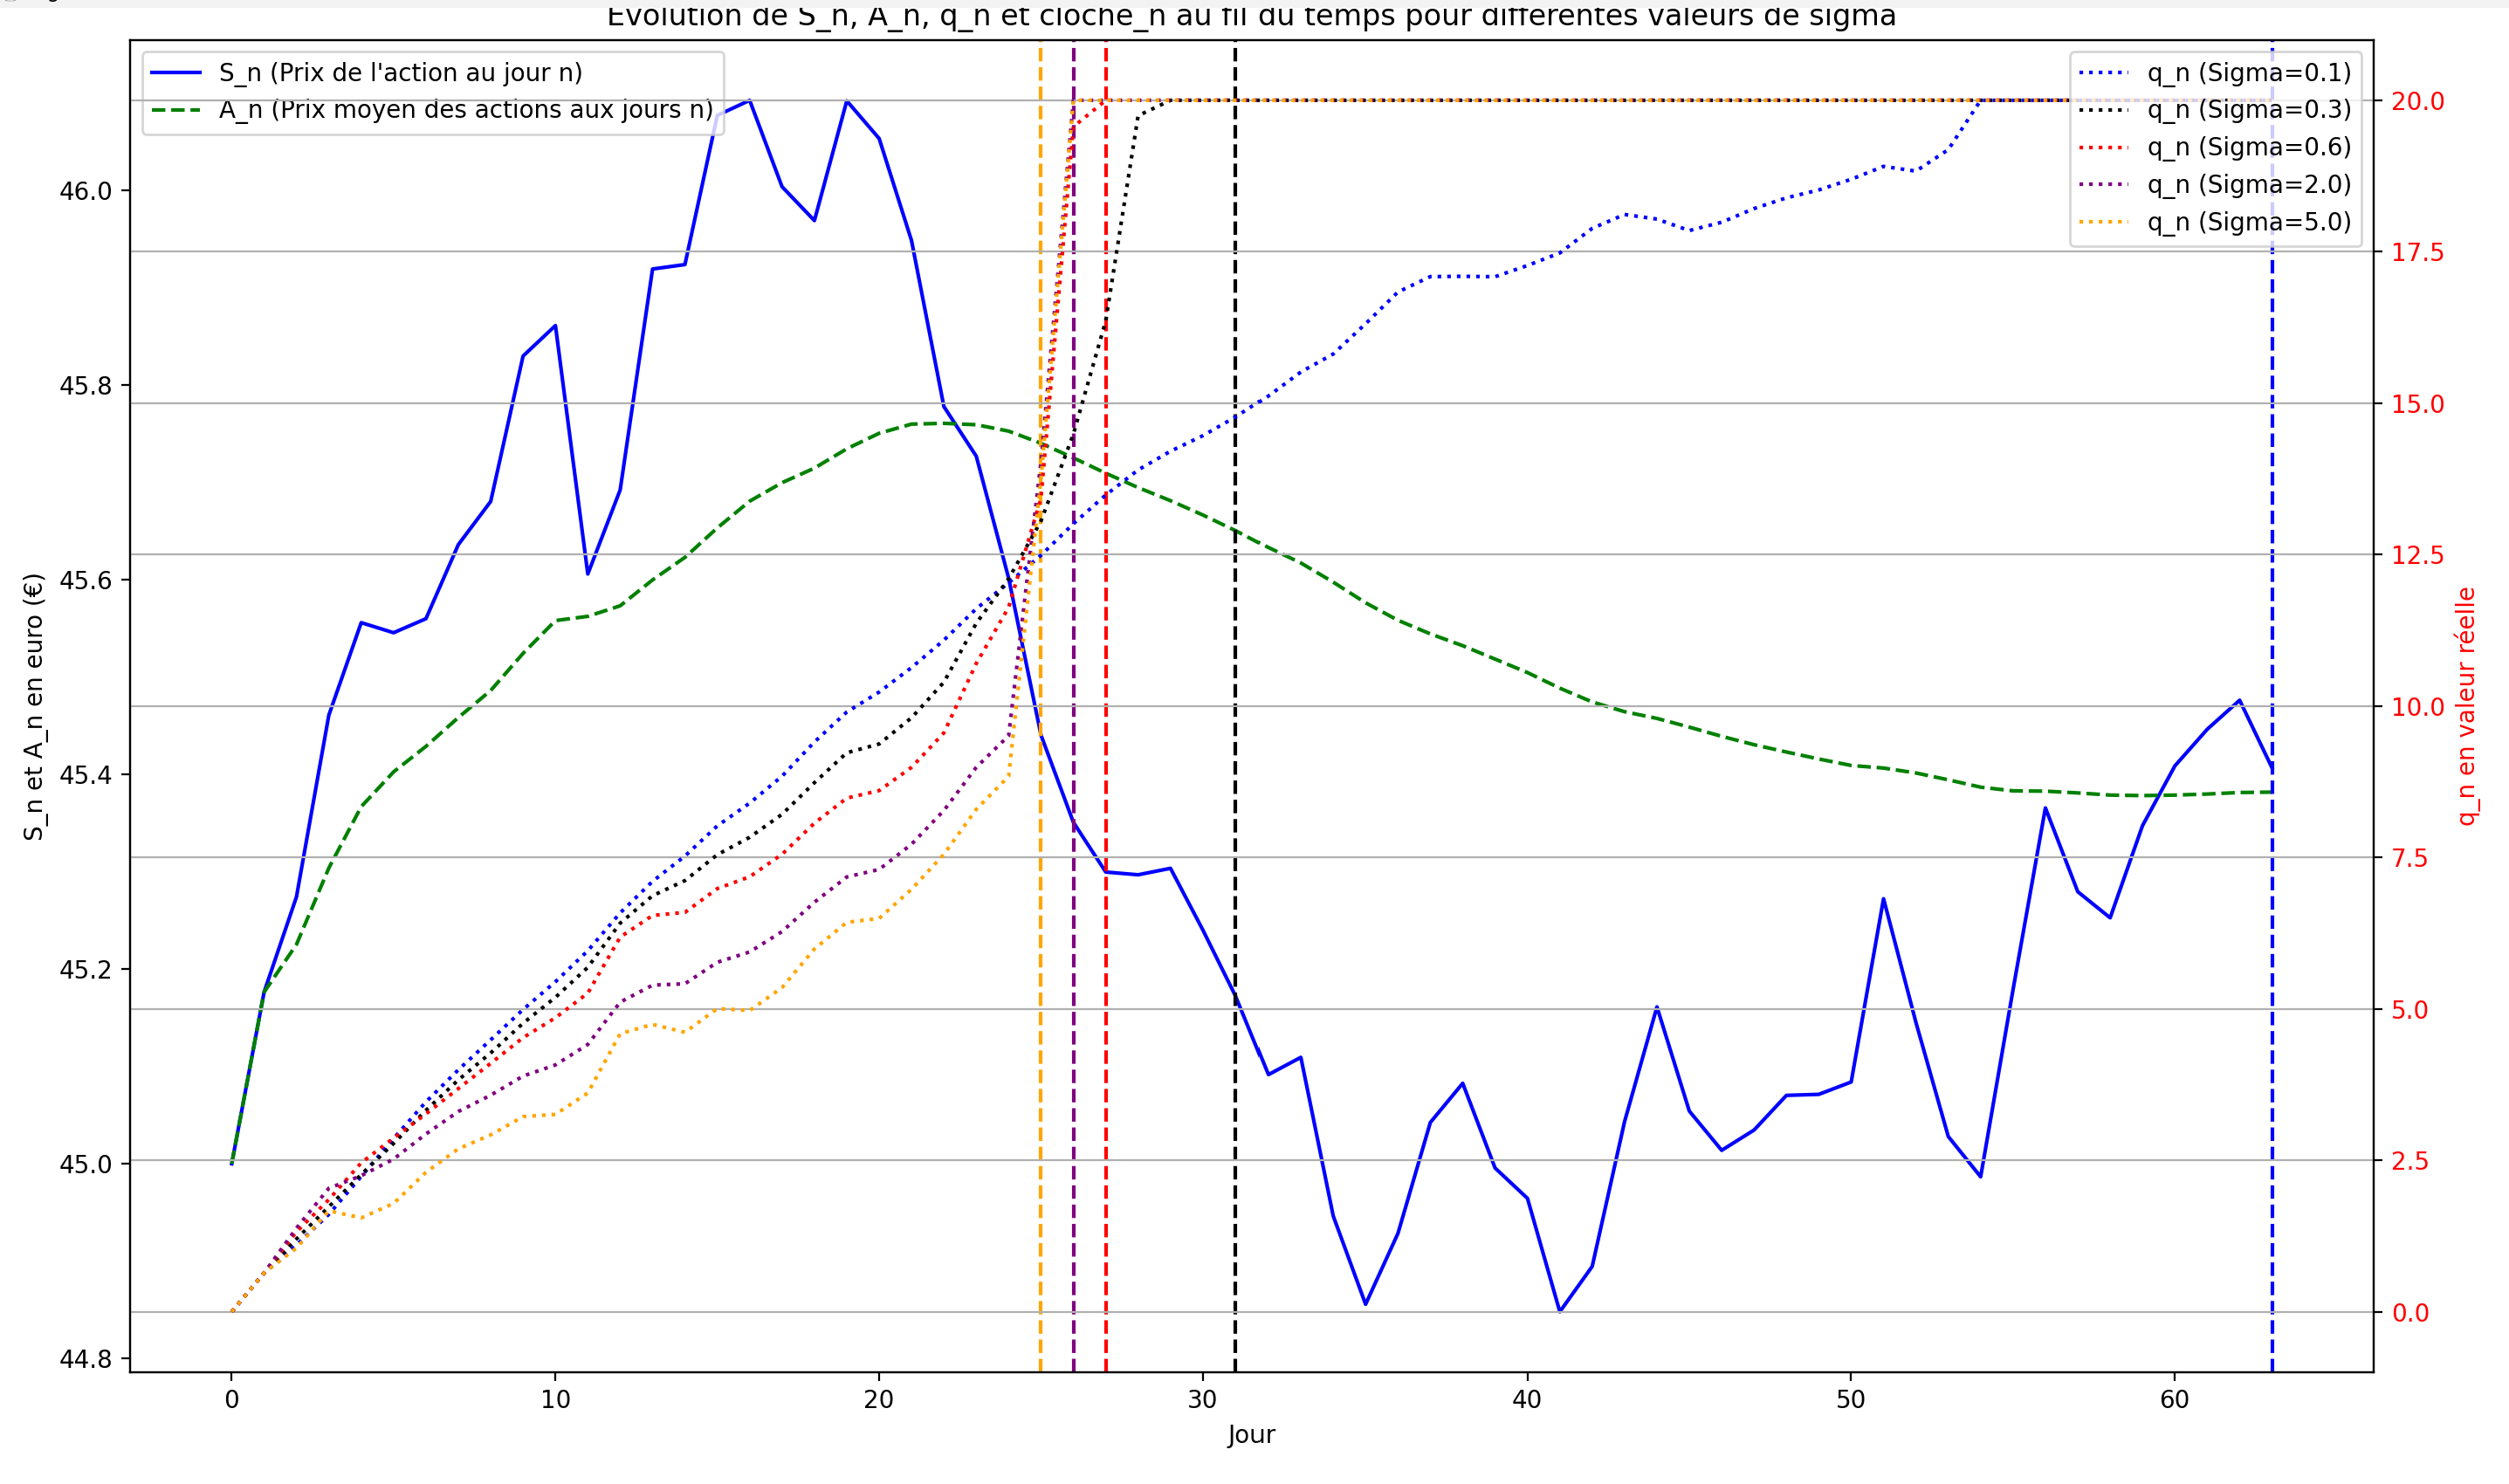
\includegraphics[width=1\textwidth]{volatilite.png}
    \caption{Impact of varying volatility on the stock buyback process and agent's decisions.}
\end{figure}


\section{Discussion}
Initial simulations revealed several promising results and issue:
\begin{itemize}
    \item The agent implemented in \texttt{nn.py} with the pre-trained model \texttt{trained\_model.pt} produces positive payoffs across our environment regardless of the seed used.
    \item The model's convergence is unstable depending on the learning rate.
    \item At first, the agent did not always achieve its purchase objective within the allotted time. However, this issue was resolved by removing the short-selling option, which simplified the process and made it easier to reach the goal.
    \item To improve the model, the following methods were attempted:
    \begin{itemize}
        \item Normalizing input variables to stabilize learning.
        \item Adjusting the learning rate for better stability.
        \item Modifying initial variables to generate different outcomes.
        \item Experimenting with different reward structures to improve decision-making.
        \item Recursive payoff computation to calculate dynamically the payoff for better stability of the learning.
    \end{itemize}
\end{itemize} 
\section{Conclusion}
Various approaches are possible to address the identified issues:
\begin{itemize}
    \item Variance reduction via a Critic and regularization, as well as direct optimization of the policy or alternating learning of the value function (critic) and optimal control (actor) (see [7]).
    \item Adjusting the learning rate and improving the learning for better stability. 
    \item Enhancing the normalization of input variables for greater stability.
    \item Experimenting with different reward structures to better guide suboptimal decision-making.
\end{itemize}

However, the results remain inconclusive and require further refinement.

We have established an experimental framework leveraging reinforcement learning to optimize a share buyback strategy. Despite significant progress, training instability and challenges in generalizing the optimal policy remain major obstacles.

Next steps include:
\begin{itemize}
    \item Enhancing training stability by exploring hyperparameters more comprehensively.
    \item Incorporating a stochastic volatility model to better reflect market conditions. [This environment was developed earlier but was set aside to focus on other optimizations using the initial setup.]
    \item Improving pre-training techniques to refine the model and avoid suboptimal decision-making by removing early incentives for hedging. This will be tested across different payoff scenarios to better guide the learning process and improve robustness. Even if it does not theoretically ensure the convergence towards a global optimum [14]
\end{itemize}

\begin{thebibliography}{9}

\bibitem{ref1}
Richard S. Sutton \& Andrew G. Barto. Reinforcement Learning An Introduction (2nd Edition).

\bibitem{ref2}
Oliver Wallscheid, Paderborn University. Lecture: Stochastic Policy Gradient Methods

\bibitem{ref3}
David Silver, DeepMind. Lecture: Policy Gradient Methods

\bibitem{ref4}
Chen, Alvin and Obizhaeva, Olga, Stock Buyback Motivations and Consequences: A Literature Review (February 9, 2022)

\bibitem{ref5}
Grullon, G., and D. L. Ikenberry. 2000. “What Do We Know about Stock
Repurchases?” Journal of Applied Corporate Finance 13 (1): 31–51. https://doi.org/10.1111/j.1745-6622.2000.tb00040.x

\bibitem{ref6}
Jiequn Han, Arnulf Jentzen, and E Weinan. Solving high-dimensional partial differential equations using deep learning. Proceedings of the National Academy of Sciences,
115(34):8505–8510, 2018

\bibitem{ref7}
Mohamed Hamdouche, Pierre Henry-Labordere and Huyen Pham. Policy gradient learning methods for stochastic control with exit time and applications to share repurchase pricing 

\bibitem{ref8}
Bastien Baldacci, Philippe Bergault, Olivier Guéant, 2024. Dispensing with optimal control: a new approach for the pricing and management of share buyback contracts

\bibitem{ref9}
Tao-Hsien Dolly King, Charles E. Teague. Accelerated share repurchases: value creation or extraction

\bibitem{ref10}
Kurt, Ahmet C., Managing EPS and Signaling Undervaluation as a Motivation for Repurchases

\bibitem{ref11}
Olivier Guéant. The Financial Mathematics of Market Liquidity: From optimal execution
to market making, volume 33. CRC Press, 2016.

\bibitem{ref12}
Olivier Guéant. Optimal execution of ASR contracts with fixed notional. Journal of
Risk, 19(5):77–99, 2017.

\bibitem{ref13}
Olivier Guéant, Jiang Pu, and Guillaume Royer. Accelerated share repurchase: pricing and execution strategy. International Journal of Theoretical and Applied Finance,
18(03):1550019, 2015.

\bibitem{ref14}
Olivier Guéant, Iuliia Manziuk, Jiang Pu. Accelerated Share Repurchase and other buyback programs: what neural networks can bring



\end{thebibliography}
\end{document}